\chapter{Construction}
\label{chapter:construction}
This chapter describes the implementation of the applications studied in the
experiments. The experiments and their results are described in
\ref{chapter:experiments}. First the common idea behind the video filtering
applications is explained and the filters used are described. After that the
PREESM and OpenEM filter applications are introduced and last the PSE model of
the OpenEM filter application is explained. This chapter is focused on the
design and implementation of the applications.

\section{Filter Application}
\label{sec:filterapp}
The objective of this thesis is to study the suitability of OpenEM framework
for stream processing. Today many different types of data can be streamed, for
example audio and video. Video was chosen to be the type of the streams used in
the experiments because there are many known image processing algorithms to use
as the basis for the study and there are many applications for video stream
processing in the context of industrial internet. TODO: ????

Three requirements for the workload applications were specified to guide the
design. The requirements are presented in the following list.

\begin{enumerate}
    \item{Variable input bitrates}
    \item{Comparability the PREESM and OpenEM applications}
    \item{Highly analyzable}
\end{enumerate}

\textbf{Variable input bitrates} were required of the workload applications to
make it possible to study the performance of the OpenEM framework in processing
dynamic workloads. Varying the bitrates of the video stream inputs is simple as
the frame size of the stream is easy to change and it doesn't affect the
algorithms used in any unforeseeable way. \textbf{Comparability of the PREESM
and OpenEM applications} was required so the PREESM workload could be used as a
baseline implementation. Last requirement for the applications was that they
needed to be \textbf{highly analyzable} in order to enable the study of OpenEM
performance. An application satisfying these requirements was designed using the
PREESM sobel example at \cite{preesmtut} as the starting point and adding
another processing component to it.

The idea for using sobel and gauss filters in the same application came from
the canny edge detector, which is briefly discussed in \ref{subsec:canny}. The
canny edge detector only provided ideas of what a realistic video processing
application does. The filters in the workload applications are executing
independently of each other on separate video streams unlike how they are
connected in the canny edge detector. After the introduction to edge detection
and the canny edge detector the filter components implemented in this thesis are
introduced in \ref{subsec:gauss} introducing the gaussian filter and
\ref{subsec:sobel} providing an overview on the sobel filter.\\

TODO: improve intro and find sources for claims. wikipedia on edge detection has
about the same stuff as above.

\subsection{Canny edge detector}
\label{subsec:canny}
Edge detection is an important tool in image processing and computer vision.
Many image processing and computer vision algorithms operate on detected edges.
There is a growing interest in the industry to use DSP platforms for edge
detection based algorithms.

In his 1986 paper John F. Canny \cite{canny1986computational} lays out the
mathematical criteria for successful edge detection and presents an algorithm,
which is suitable for implementation on DSP platforms and achieves decent edge
detection performance. The Canny Edge Detection consists of five steps
presented in the following list.

\begin{enumerate}
    \item{Noise reduction}
    \item{Finding the intensity gradient of the image}
    \item{Non-maximum supression}
    \item{Double tresholding}
    \item{Edge tracking by hysteresis}
\end{enumerate}

The noise reduction in step one can be implemented with gaussian filtering.
Finding the intensity gradient of the image in step two can be implemented using
a sobel filter. Gauss and sobel filters are implemented in the thesis
experiment. Gaussian filtering is discussed in \ref{subsec:gauss} and sobel
filtering in \ref{subsec:sobel}.  The rest of the steps are not implemented in
this thesis and thus are only briefly discussed here.

In the canny edge detector the image is first filtered with gaussian filter to
reduce the amount of noise in the image. Second the changes in the intensity in
the image are detected using an edge detection operator such as the sobel
operator. The third step improves the accuracy of the edge detection by
supressing all but the strongest responses to the detected edges, in practice
``thinning'' the edges. The fourth step classifies the edge pixels to three
classes separated by empirically determined threshold values. The pixels with
gradient value above the high threshold are marked strong pixels and the pixels
with gradient value below the low threshold are supressed. In the fifth step the
remaining weak pixels with gradient values below the high threshold are
preserved or supressed according to the presence of strong pixels in their
neighborhood. Detailed description of the algorithm is presented in the original
paper by Canny \cite{canny1986computational}, information about implementing a
canny edge detector is available in \cite{gonzalez2008digital} and comparison of
its performace to other edge detectors can be found in \cite{maini2009study}.

\subsection{Gaussian filter}
\label{subsec:gauss}
Gaussian filtering is used for multiple purposes in digital image processing.
In canny edge detector the gaussian filter is used to reduce noise in the
processed images. The gaussian filter works by convolving a gaussian function
with the input signal. Gaussian function is non-zero everywhere which means it
would theoretically require an infinite convolution window. Since the function
decays rapidly it is often reasonable to truncate the function and use small
windows. \cite{gonzalez2008digital} In the thesis experiment a kernel size of
5x5 is used. In practice every pixel in the filtered image has an intensity
value computed by taking a weighted average of the neighboring pixels in the
input image. The weights are precalculated from the gaussian function, giving
the highest weight to the pixel in the center of the window. The gaussian
function was calculated with $\sigma$ = 1.3. The filtered image has a smoothed
appearance compared to the original image.

\subsection{Sobel filter}
\label{subsec:sobel}
The actual edge detection in the canny edge detector starts with applying the
sobel operator on the input image. The sobel operator is a discrete
differentiation operator. It consists of two 3x3 kernels which are convolved
with the image to approximate the derivatives. The two kernels represent
horizontal and vertical changes. At each point in the image the resulting
gradient approximations are combined giving an approximate gradient magnitude.
\cite{gonzalez2008digital}

\section{PREESM Filter Application}
\label{sec:preesmapp}
An actor network is constructed in PREESM that represents the video filter
application. The final PiSDF model of the PREESM video filter application is
presented in figure \ref{preesm_actors}. The PREESM filter application is
adapted from the PREESM tutorial at \cite{preesmtut} by adding another
processing path for gaussian filter and making the necessary modifications to
the shared parts of the application.

\begin{figure}[h!] \label{preesm_actors} \begin{center}
    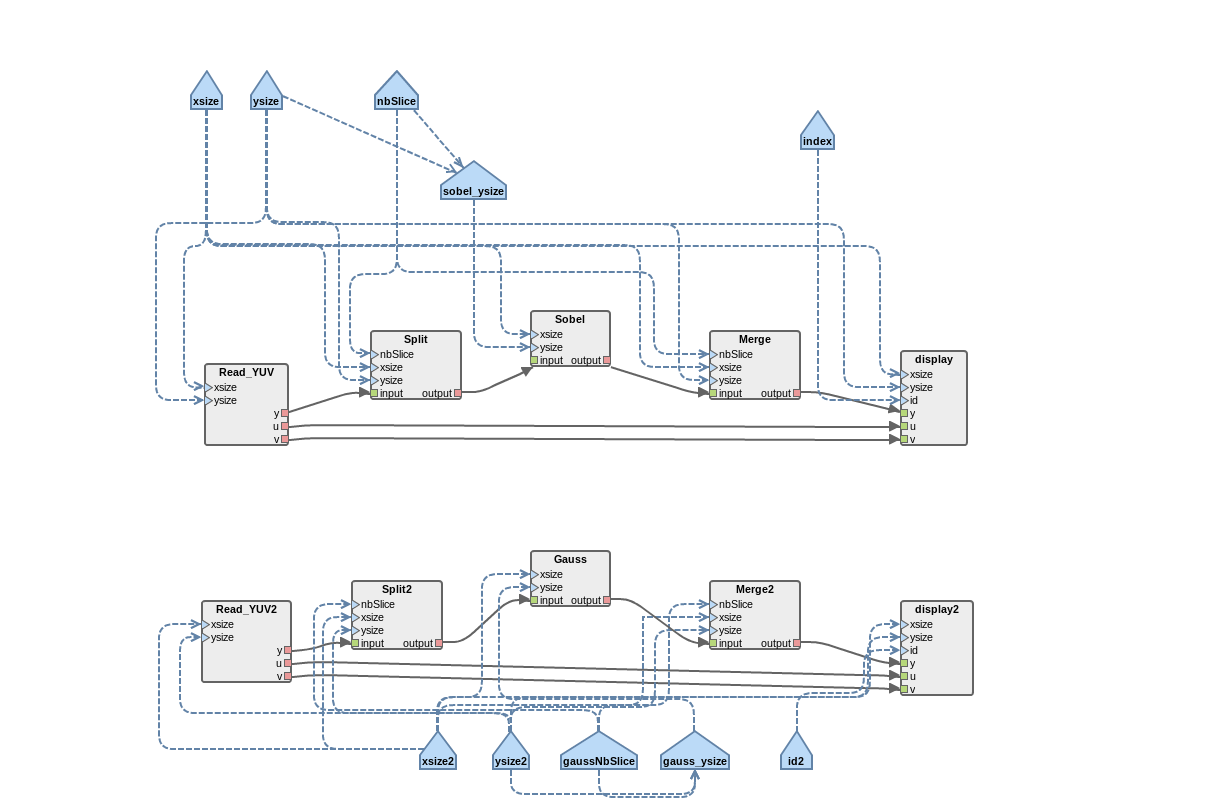
\includegraphics[width=0.99\textwidth]{images/preesm_diagram.png}
    \caption{The PiSDF graph of the PREESM filter application} \end{center}
\end{figure}

To keep the model simple and the program well analyzable both of the processing
paths in the network are independent.

The first actor on both of the processing paths loads the video frames from
memory and passes them to splitting actors. The splitting actor splits the
frames to a suitable number of splices to enable processing of the same video
stream on multiple cores. The filter actor follows the splitting actor. Partial
frames filtered in the filter actor are merged back to whole frames in the merge
actors. The last actors on both of the processing paths are dummy actors.\\

TODO: explain scheduling

\section{OpenEM Filter Application}
The OpenEM implementation of the filter application was heavily influenced by
the PREESM filter application described in \ref{sec:preesmapp}. Specifically the
OpenEM application has to process the frames in similar manner so that only the
scheduling policies between the two programming models should differ. The PREESM
application splits the frames into slices and processes the slices separately
before merging them back into one frame. Similar fork-join mechanism was
implemented in the OpenEM application. Event groups were first planned to be
used as the fork-join mechanism in the filter application but in the final
implementation a different, simpler mechanism was used.

The TI implementation of event groups lacks \texttt{em\_event\_group\_delete}
function which makes it necessary to reuse the existing event groups. The
example applications which are included in the NSN OpenEM distribution
described in \ref{sec:emframework} demonstrate reuse of event groups, but it
was estimated that the programming overhead resulting from the reuse of the
groups would be larger than implementing the fork-join in a simpler manner.

In the final implementation the frames are accumulated simply in a merge buffer
located in shared memory which is referenced through queue context pointers. The
book keeping for frame completion is handled in the same location. The cache
coherency for the book keeping was handled by marking the memory area the merge
buffer resides in as non-cacheable.

\section{PSE Model of OpenEM Filter Application}
\section{Instrumentation}
